
\subsection{Adapter-System}

\subsubsection{Aufgaben}
Da bei der API viel Wert auf Flexibilität gelegt wird, sollte die Bibliothek in der Lage sein mit den verschiedensten Steuerungen zu kommunizieren. Es soll ein System entwickelt werden mit dem die API zukünftig auch auf neue Steuerungen erweiterbar ist. Im Rahmen der Diplomarbeit soll die Kommunikation mit der KEBA- und der GHI-Steuerung ermöglicht werden. Weiters wird für die Visualisierung in der Endanwendung eine Art "'virtuelle Steuerung"' benötigt.

\subsubsection{Aufbau}
Die Grundidee besteht darin, den zukünftigen Anwendern eine einfache Erweiterung der API um neue Steuerungssysteme zu ermöglichen. Um diese Idee zu realisieren wird ein Adapter-System verwendet, bei der für jede Steuerung ein Adapter als Schnittstelle dient. Um einen neuen Adapter zu implementieren muss lediglich eine Klasse implementiert werden, die von der abstrakten \textit{IAdapter}-Klasse abgeleitet ist. Ein Objekt dieser abgeleiteten Klasse kann dann bei der \textit{Edubot}-Klasse mit Hilfe der \textit{RegisterAdapter-Methode} registriert werden. Der Adapter dient dann als Übersetzer der allgemeinen Befehle in die spezifischen Steuerungssprachen und kümmert sich um die Beschaffung beziehungsweise Berechnung potentiell benötigter, zusätzlicher Informationen. Die in den darauffolgenden Kapiteln vorgestellten Adapter  \textit{EdubotAdapter}, \textit{KebaAdapter} und \textit{VirtualAdapter} sind ebenfalls von dieser \textit{IAdapter}-Klasse abgeleitet und dienen als Demonstration der Funktionalität dieses Systems. 

\subsubsection{Umsetzung}

Da die Umsetzung dieses System relativ umfangreich ist, wurde es nochmals in die folgenden, im weiteren Verlauf beschriebenen, Bereiche unterteilt.\\

\textbf{Der Grundbaustein "'IAdapter"'}\\
Jeder Adapter muss die abstrakte Klasse \textit{IAdapter} implementieren, welches alle Grundinformationen bezüglich des angeschlossene Steuerung und des dazugehörigen Roboters enthält. Weiters müssen alle vorhandenen Kommandos von den Adaptern unterstützt werden, weshalb für jedes Kommando eine entsprechende Methode im \textit{IAdapter} vorhanden ist. Diese Klasse besitzt folgende Properties:
\begin{itemize}
\item \textbf{Length}\\
Gibt die Länge der ersten Roboterachse, gemessen an der Distanz zwischen dem Mittelpunkt der ersten und zweiten der Motorwelle, an. Die Längenangabe kann dabei in einer beliebigen Einheit sein, da es bei der Berechnung lediglich auf das Verhältnis der beiden Roboterachsen ankommt.
\item \textbf{Length2}\\
Gibt die Länge der zweiten Roboterachse an, gemessen an der Distanz zwischen dem Mittelpunkt der zweiten Motorwelle und dem Werkzeugmittelpunkt, an. Für die korrekte Pfadberechnung muss dieser Wert in derselben Einheit wie "'Length"' angegeben sein.
\item \textbf{VerticalToolRange}\\
Gibt die Distanz zwischen dem Werkzeugmittelpunkt und der Arbeitsfläche an, wenn sich das Werkzeug an der höchstmöglichen Position befindet. Für die korrekte Pfadberechnung muss dieser Wert in derselben Einheit wie "'Length"' angegeben sein.
\item \textbf{Transmission}\\
Gibt an um wie viel Grad sich der Motor der transversalen Achse drehen muss, um diese eine Einheit (z.B.: Millimeter) nach unten zu verschieben.
\item \textbf{MaxPrimaryAngle}\\
Gibt den Maximalwinkel an, den die erste Achse einnehmen kann. Dieser ist bei Robotermodellen, wie zum Beispiel dem Edubot-Modell, abhängig von der Bauweise. Soll der Maximalwinkel nicht berücksichtigt werden, weil es sich zum Beispiel um einen virtuellen Adapter handelt, so wird empfohlen diesen Wert auf float.MaxValue festzulegen.
\item \textbf{MinPrimaryAngle}\\
Gibt den Minimalwinkel an, den die erste Achse einnehmen kann. Dieser ist bei Robotermodellen, wie zum Beispiel dem Edubot-Modell, abhängig von der Bauweise. Soll der Minimalwinkel nicht berücksichtigt werden, weil es sich zum Beispiel um einen virtuellen Adapter handelt, so wird empfohlen diesen Wert auf float.MinValue festzulegen.
\item \textbf{MaxSecondaryAngle}\\
Gibt den Maximalwinkel an, den die zweite Achse einnehmen kann. Dieser ist bei Robotermodellen, wie zum Beispiel dem Edubot-Modell, abhängig von der Bauweise. Soll der Maximalwinkel nicht berücksichtigt werden, weil es sich zum Beispiel um einen virtuellen Adapter handelt, so wird empfohlen diesen Wert auf float.MaxValue festzulegen.
\item \textbf{MinSecondaryAngle}\\
Gibt den Minimalwinkel an, den die zweite Achse einnehmen kann. Dieser ist bei Robotermodellen, wie zum Beispiel dem Edubot-Modell, abhängig von der Bauweise. Soll der Minimalwinkel nicht berücksichtigt werden, weil es sich zum Beispiel um einen virtuellen Adapter handelt, so wird empfohlen diesen Wert auf float.MinValue festzulegen.
\item \textbf{Result}\\
Diese Eigenschaft beinhaltet das Ergebnis der letzten Pfadberechnung in Form eines InterpolationResult-Objekts. Ob das Result-Property bei einem Adapter einen Wert enthält, kommt darauf an ob er die Pfadkalkulation der API verwenden. 
\item \textbf{CmdQueue}\\
Bei der\textit{CmdQueue} handelt es sich um eine Warteschlange mit anstehenden Befehlen für die Steuerung, die in der Reihenfolge in der sie ankommen abgearbeitet werden. Die Liste besteht aus Elementen des Typs \textit{ICommand} (siehe Kommando-System), welche mit der \textit{Execute}-Methode ausgeführt werden.\\
Der Grund für die separate Verwaltung der anstehenden Befehle in jedem Adapter liegt darin, dass jeder Roboter eine unterschiedliche lange Zeitdauer zum Ausführen eines Befehls benötigt.
\end{itemize}

\begin{figure}[H]
  \centering
  \begin{minipage}[t]{12 cm}
  	\centering
  	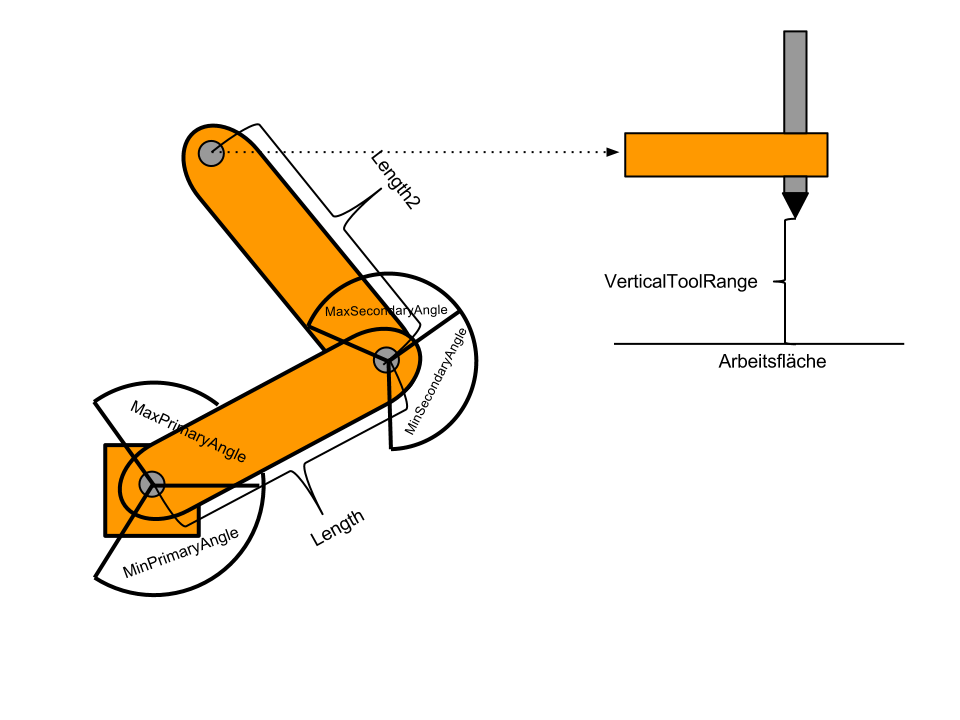
\includegraphics[width=12cm]{images/AdapterProperties} 
    \caption{Bedeutung der IAdapter-Properties}
  \end{minipage}
\end{figure}

\textbf{Konstruktoren}\\
Die IAdapter-Klasse besitzt vier vorgegebene Konstruktoren, von denen eine abgeleitete Klasse mindestens einen verwenden muss. Die jeweiligen Konstruktoren sind auf verschiedene Bauweisen eines Roboters mit RR beziehungsweise RRT zugeschnitten.
\begin{itemize}
\item \textbf{RR-Kinematik ohne Winkelbeschränkungen}\\
Diesem Konstruktor werden lediglich die Längen der beiden Achsen mitgegeben. Durch die Bauweise des Roboters vorhandene Winkeleinschränkungen werden bei Pfadberechnung nicht berücksichtigt.
\item \textbf{RR-Kinematik mit Winkelbeschränkungen}\\
Diesem Konstruktor werden die Längen der beiden Achsen sowie die jeweiligen Winkeleinschränkungenen mitgegeben. Durch die Bauweise des Roboters vorhandene Winkeleinschränkungen werden bei Pfadberechnung berücksichtigt.
\item \textbf{RRT-Kinematik ohne Winkelbeschränkungen}\\
Diesem Konstruktor werden die Längen der beiden Achsen, die Distanz zwischen Toolcenter-Point und Arbeitsfläche sowie die Übersetzung der transversalen Achse mitgegeben. Durch die Bauweise des Roboters vorhandene Winkeleinschränkungen werden bei Pfadberechnung nicht berücksichtigt.
\item \textbf{RRT-Kinematik mit Winkelbeschränkungen}\\
Diesem Konstruktor werden die Längen der beiden Achsen, die Distanz zwischen Toolcenter-Point und Arbeitsfläche, die Übersetzung der transversalen Achse sowie die jeweiligen Winkeleinschränkungenen mitgegeben. Durch die Bauweise des Roboters vorhandene Winkeleinschränkungen werden bei Pfadberechnung berücksichtigt.
\end{itemize}

\textbf{Status eines Adapters}\\
Die wohl wichtigste Information über einen Adapter ist in der geschützten Variable \textbf{state} enthalten. Diese gibt Auskunft über den aktuellen Zustand des Roboters mit Hilfe der \textit{State}-Enumeration der API. Dieser Wert ist nur in der IAdapter-Klasse und von ihr abgeleiteten Klassen sichtbar, da sie grundsätzlich nur über die Methode \textit{SetState} geändert werden sollte.\\
Um den aktuellen Zustand zu erhalten beziehungsweise diesen zu verändern, werden folgende Methoden bereitsgestellt:
\begin{itemize}
\item \textbf{GetState}\\
Bei Aufruf dieser Methode wird der aktuelle Zustand des Adapters in Form eines State-Objekts zurückgegeben.
\item \textbf{SetState}\\
Diese Methode ist zwei mal überladen und stellt die empfohlene Vorgehensweise zum Ändern der \textit{state}-Variable dar.\\
Die erste Variante der Methode übernimmt als Parameter lediglich den neuen Zustand. Zu Beginn wird mittels der \textit{IsStateUpdateAllowed}-Methode geprüft ob manuelle Zustandsupdates überhaupt erlaubt sind. Die soeben erwähnte Methode muss von jeder, von IAdapter abgeleiteten, Klasse implementiert werden. Liefert diese \textit{true} zurück so wird \textit{UpdateState} aufgerufen, andernfalls wir das OnFailure-Event mit Hilfe der RaiseFailureEvent-Methode ausgelöst.\\
Die zweite Variante der \textit{SetState}-Methode übernimmt zusätzlich zum neuen Zustand, einen boolschen Wert, welcher angibt ob die Bedingungen zum Ändern des Zustands ignoriert werden sollen. Bei Verwendung dieser Methode außerhalb ist Vorsicht geboten, da durch falsche Verwendung der jeweilige Adapter nicht mehr richtig arbeiten könnte. Diese Variante wird lediglich zum Aktualisieren des Zustands eines Edubot- beziehungsweise KebaAdapter-Objekts durch deren Listener und die von uns implementierten Befehle verwendet.
\item \textbf{UpdateState}\\
Die UpdateState-Methode übernimmt die eigentliche Änderung der Variable indem sie letztere auf den, als Parameter mitgegebenen, Wert setzt. Zuvor löst sie allerdings noch das OnStateChanged-Event aus, welchem der alte und neue Zustand in den Event-Argumenten übergeben wird. Zuletzt wird noch die \textit{CheckState}-Methode aufgerufen, die sich um die potentiellen Auswirkungen des neuen Zustands kümmert.
\item \textbf{CheckState}\\
Nachdem die \textit{state}-Variable geändert wurde, muss diese überprüft werden, da gewisse Zustände zur Ausführung des nächsten Befehls aus der \textit{CmdQueue} führen können. Bei Aufruf dieser Methode wird geprüft ob sich der Adapter im Zustand \textit{READY} oder \textit{SHUTDOWN} befindet und sich Befehle in der Warteschlange befinden. Treffen diese Bedingungen zu, so wird das nächste ICommand-Objekt (siehe Kommando-System) herausgeholt und mit dessen \textit{CanExecute}-Methode geprüft ob der Befehl selbst ausgeführt werden kann. \\
Sollte die Durchführung des Befehls nicht möglich sein, wird von der zuletzt erwähnten Methode ein \textit{FailureEventArgs}-Objekt zurückgegeben und das \textit{OnFailureEvent} durch Aufruf von \textit{RaiseFailureEvent} ausgelöst. Andernfalls wird der Befehl mit Hilfe seiner \textit{Execute}-Methode ausgeführt.

\begin{lstlisting}[language = CSharp, captionpos=b, caption={Die CheckState-Methode des IAdapters}]
private void CheckState()
        {
            if ((state == State.READY || state == State.SHUTDOWN) && cmdQueue.Count > 0)
            {
                ICommand nextCmd = cmdQueue.Dequeue();
                FailureEventArgs failureArgs = nextCmd.CanExecute(this);
                if (failureArgs == null)
                {
                    nextCmd.Execute(this);
                }
                else
                {
                    RaiseFailureEvent(failureArgs);
                }
            }
        }
\end{lstlisting}
\end{itemize}

\textbf{Ausführen von Befehlen}\\
Die nachstehende Methode {Execute} wird ebenfalls vom IAdapter implementiert, da sie sich grundsätzlich nur um das Einreihen von Befehlen in die Warteschlange und nicht um die eigentliche Durchführung der Befehle kümmert.
\begin{itemize}
\item \textbf{Execute}\\
Diese Methode übernimmt ein \textit{ICommand}-Objekt als Parameter. Zuerst wird überprüft ob es sich bei dem Objekt um ein Objekt vom Typ \textit{AbortCommand} handelt, da dieser Befehl der einzige ist, der aus sicherheitstechnischen Gründen unverzüglich nach Eintreffen ausgeführt werden muss. Befehle anderer Art, werden mit Hilfe der \textit{Enqueue}-Methode in die Warteschlange gegeben. Anschließend wird \textit{CheckState} aufgerufen, welche bereits weiter oben erklärt wurde.\\

\end{itemize}

\begin{lstlisting}[language = CSharp, captionpos=b, caption={Die Execute-Methode des IAdapters}]
public void Execute(ICommand cmd) {
            if (cmd is AbortCommand)
            {
                cmd.Execute(this);
            }
            else
            {
                cmdQueue.Enqueue(cmd);
                CheckState();
            }
        }
\end{lstlisting}


\textbf{Kollisionsvermeidung und Punktvalidierung}\\
Da ein realer Roboterarm nur über eine begrenzte Reichweite verfügt, wird mit Hilfe der hier angeführten Methoden während der Interpolation die Gültigkeit von Punkten und Winkeln geprüft.
\begin{itemize} 
\item \textbf{IsPointValid}\\
In dieser Methode wird überprüft ob ein, der Methode als Parameter mitgegebener, Punkt vom Adapter überhaupt erreicht werden kann. Dazu wird im wesentlichen überprüft ob die Distanz vom Koordinatenursprung zum Zielpunkt kleiner oder gleich der Gesamtlänge der beiden Achsen ist. Die Z-Koordinate muss zwischen 0 und der vertikalen Reichweite des Werkzeugs liegen, um als gültig angesehen zu werden. Erfüllt der Punkt diese Voraussetzungen so kann er vom Roboter erreicht werden, weshalb die Methode true zurückliefert.
\item \textbf{AreAnglesValid}\\
Diese Methode dient der Kollisionsvermeidung und überprüft ob die, als Parameter übergebenen, Achswinkel gültig sind. Dabei kommen die Properties \textit{MaxPrimaryAngle}, \textit{MinPrimaryAngle}, \textit{MaxSecondaryAngle} und \textit{MinSecondaryAngle} zum Einsatz. Ob der Winkel der Z-Achse gültig ist, wird mit Hilfe des \textit{VerticalToolRange}-Properties in Kombination mit dem \textit{Transmission}-Property überprüft. Liegt einer der mitgegebenen Winkel nicht im gültigen Bereich, so liefert die Methode false zurück.
\end{itemize}

\textbf{Abstrakte Methoden}\\
Im Anschluss werden die abstrakten Methoden vorgestellt die von den abgeleiteten Klassen implementiert werden müssen. Hierbei handelt es sich um eine allgemeine Erklärung des Zwecks, da auf die genaue Implementierung in den Kapiteln zu den verschiedenen Adaptern eingegangen wird. Da die meisten der angegebenen Methoden aus Performance-Gründen in einem eigenen Thread ausgeführt werden, handelt es sich bei den Parametern immer um Objekte vom Typ \textit{object}. 
\begin{itemize}
\item \textbf{Initialize}\\
Diese Methode wird während der Ausführung der \textit{Execute}-Methode eines \textit{StartCommand}-Objekts ausgeführt. In dieser Methode sollen alle nötigen Vorbereitungen zum Betrieb der Steuerung beziehungsweise des Roboters getroffen werden. Vor allem sollte hier die Steuerung mit dem Homing, einem Algorithmus der den Roboter in eine bestimmte Ausgangsposition bringt, beginnen.
\item \textbf{Shutdown}\\
Diese Methode wird während der Ausführung der \textit{Execute}-Methode eines \textit{ShutdownCommand}-Objekts ausgeführt. Sie sollte zum geplanten Herunterfahren des Roboters dienen und sollte nach erfolgreichen Durchführung den Roboter in ausgeschaltetem Zustand hinterlassen.
\item \textbf{MoveStraightTo}\\
Diese Methode wird während der Ausführung der \textit{Execute}-Methode eines \textit{MVSCommand}-Objekts ausgeführt. Es erhält als Parameter den angesteuerten Zielpunkt in Form eines \textit{Point3D}-Objekts. Abhängig davon, worauf das \textit{RequiresPrecalculation-Property} gesetzt wurde, ist der Pfad zu diesen Zeitpunkt bereits berechnet und ist im Adapter in Form eines \textit{InterpolationResult}-Objekts zur weiteren Verwendung vorhanden. Aufgabe dieser Methode ist das Durchführen einer linearen Bewegung vom aktuellen Werkzeugmittelpunkt zum Zielpunkt.
\item \textbf{MoveCircularTo}\\
Diese Methode wird während der Ausführung der \textit{Execute}-Methode eines \textit{MVCCommand}-Objekts ausgeführt. Es erhält als Parameter ein \textit{Point3D}-Array mit 2 Punkten - dem angesteuerten Zielpunkt am Index 0 und den angegebenen Mittelpunkt am Index 1. Auch hier ist es wieder abhängig davon, ob das \textit{RequiresPrecalculation}-Property gesetzt wurde, ob eine \textit{InterpolationResult}-Objekt aus der Pfadberechnung vorhanden ist. Aufgabe dieser Methode ist das Durchführen einer zirkularen Bewegung unter Verwendung des angegebenen Mittelpunkts.
\item \textbf{UseTool}\\
Diese Methode wird während der Ausführung der \textit{Execute}-Methode eines \textit{UseToolCommand}-Objekts ausgeführt. Sie erhält als Parameter einen boolschen Wert, der angibt ob das Werkzeug aktiviert oder deaktiviert werden soll. Je nach Wert werden benötigte Informationen an den Roboter weitergegeben und dadurch das jeweilige Werkzeug aktiviert.
\item \textbf{Abort}\\
Diese Methode wird während der Ausführung der \textit{Execute}-Methode eines \textit{AbortCommand}-Objekts ausgeführt. Diese Methode dient als eine Art Software-Endschalter und sollte den Roboter, unabhängig von seiner aktuellen Aktion, auf der Stelle anhalten und ausschalten. 
\item \textbf{IsStateUpdateAllowed}\\
Der Rückgabewert dieser Methode ist boolean und legt fest, ob der Zustand dieses Adapters von außen geändert werden darf.
\item \textbf{UsesIntegratedPathCalculation}\\
Der Rückgabewert dieser Methode ist boolean und legt fest, ob die Pfadberechnung mit Hilfe API durchgeführt werden soll. Besitzt die, mit dem Adapter angesprochene, Steuerung eigene Verfahren zur Pfadberechnung so empfiehlt sich hier \textit{false} zurückzugeben.
\end{itemize}

\textbf{VirtualAdapter}\\
Dieser Adapter stellt die simpelste Implementierung der IAdapter-Klasse dar und dient prinzipiell zur Simulation einer Steuerung. Er wird ebenso bei der Edubot-Klasse registriert und wie alle anderen Adapter behandelt mit dem Unterschied, dass er keine tatsächlichen Aktionen durchführt sondern vielmehr die richtigen Events zur richtigen Zeit auslöst. Diese Eigenschaft macht den \textit{VirtualAdapter} sehr vielseitig, weshalb er beispielsweise auch bei der Umsetzung der Visualisierung in der Endanwendung verwendet wurde.\\
\\
Bezüglich der \textit{IAdapter}-Methoden ist der \textit{VirtualAdapter} beschränkt sich der VirtualAdapter hauptsächlich auf das Aktualisieren des ToolCenterPoints. Die hier nicht angeführten Methoden der IAdapter-Klasse sind leer und erfüllen daher keine Funktion.
\begin{itemize}
\item \textbf{Initialize}
\newline
Bei Aufruf der \textit{Initialize}-Methode wird der ToolCenterPoint auf den Ausgangspunkt gesetzt.
\item \textbf{Shutdown}
\newline
Bei Aufruf der \textit{Shutdown}-Methode 
\newline
Bei Aufruf der \textit{MoveStraight}-Methode wird der ToolCenterPoint auf den Zielpunkt gesetzt.
\item \textbf{MoveCircular}
\newline
Bei Aufruf der \textit{MoveCircular}-Methode wird der ToolCenterPoint ebenfalls auf den Zielpunkt gesetzt.
\newline
\item \textbf{IsStateUpdateAllowed}\\
Durch die Möglichkeit den Zustand des Adapters von außen ändern und auf alle wichtigen Events reagieren zu können, bietet sich ein breites Anwendungsspektrum für den VirtualAdapter. Aus diesem Grund gibt diese Methode bei Aufruf immer \textit{true} zurück.
\item \textbf{UsesIntegratedPathCalculation}\\
Da hinter dem VirtualAdapter natürlich keine Steuerung steckt, ist er voll und ganz auf die Pfadberechnung der API angewiesen, weshalb diese Methode immer \textit{true} zurückliefert.
\end{itemize}


\textbf{EdubotAdapter}
\newline
Der \textit{EdubotAdapter} dient als Schnittstelle zum kleineren Modell unseres SCARA-Roboters. Er kommuniziert via Netzwerk mit der Steuerung von GHI, auf welcher eine eigens entwickelte Steuerungssoftware läuft. Der Adapter ist, wie bereits oben angemerkt, von der abstrakten \textit{IAdapter}-Klasse abgeleitet. Zusätzlich zu den geerbten Properties, enthält die Klasse noch folgende zusätzliche Properties:
\begin{itemize}
\item \textbf{Endpoint}\\
Das \textit{Endpoint}-Property beinhaltet die IP-Adresse der GHI-Steuerung, sowie den Port auf dem die Steuerungssoftware läuft. Standardmäßig läuft die Steuerungssoftware auf Port 12000. Der Endpoint wird von \textit{Connect}-Methode des Sockets zum Aufbauen einer Verbindung verwendet.
\item \textbf{Socket}\\
Um in C\# eine Netzwerkverbindung aufzubauen, werden sogenannte Sockets verwendet. Beim Erstellen einer neuen Instanz der Socket-Klasse, müssen spezifische Angaben über den Address-, Socket- und Protokolltyp im Konstruktor mitgegeben werden.\\
Als Addresstyp verwenden wir \textit{AddressFamily.InterNetwork}, da es sich dabei laut MSDN um den Typ für IPv4-Adressen handelt. Weiters werden die Daten an die Steuerung gestreamt, weshalb wir als \textit{Sockettyp SocketType.Stream} verwenden. Zuletzt muss noch der Protokolltyp angegeben werden. \\
Da bei der Übertragung des Interpolationsergebnisses keine Informationen verloren gehen dürfen, muss ein verlässliches Transport-Protokoll verwendet werden. Das Standard-Protokoll für diese Anforderungen ist das TCP (Transmission Control Protocol), welches deshalb auch als Protokolltyp angegeben wird.
Mit Hilfe dieses Sockets und dem \textit{Endpoint}-Property, ist der \textit{EdubotAdapter} in der Lage sich zur GHI-Steuerung zu verbinden.
\end{itemize}

Weiters verfügt dieser Adapter aufgrund seiner Art der Kommunikation noch die Methoden zur Kontrolle und Änderung der Netzwerkeinstellungen:
\begin{itemize}
\item \textbf{TestConnectivity}
\newline
 Bei Aufruf dieser Methode versucht der Adapter sich kurzzeitig mit der Steuerung zu verbinden. Dazu wird, wie beim Property \textit{Socket} beschrieben, ein Stream geöffnet, jedoch mit zusätzlichen Einstellungen: Die Socket-Feature "'Linger"' wird via \textit{SetSocketOption} deaktiviert. Der Hintergrund ist der, dass beim Schließen eines Sockets normalerweise die Verbindung so lange offen gehalten wird bis wartende Pakete gesendet wurden. Um dies zu gewährleisten, wartet ein Socket mit dem Linger-Feature in etwa 2 Minuten und schließt erst dann die Verbindung vollständig. Da der Sinn dieser Methode jedoch nur ein schneller Verbindungstest ist, muss dieses Feature deaktiviert werden. Weiters wird der Send- beziehungsweise Receive-Timout auf 5 Sekunden gesetzt, damit das Auslösen einer \textit{SocketException} durch den abgelaufenen Timeout nicht zu lange dauert. Die Methode gibt bei erfolgreichem Aufbauen und Trennen der Verbindung wird \textit{true}, bei Auftreten einer Exception \textit{false} zurückgegeben.
\item \textbf{SetNetworkConfiguration}
\newline
Diese Methode dient zum setzen der Netzwerkeinstellungen und übernimmt als Parameter eine IP-Addresse und eine Port-Nummer. Im nächsten Schritt prüft sie ob derzeit eine Verbindung zur Steuerung besteht. Ist dies der Fall so wird die Verbindung geschlossen. Im Anschluss werden das \textit{Socket}-Objekt, das \textit{Endpoint}-Objekt und der \textit{NetworkStateListener} neu instanziert.
\end{itemize}

Bezüglich der \textit{IAdapter}-Methoden ist der \textit{EdubotAdapter} folgendermaßen implementiert:
\begin{itemize}
\item \textbf{Initialize}
\newline
Bei Aufruf der \textit{Initialize}-Methode wird die Verbindung zur Steuerung hergestellt und ein String mit dem Inhalt "'hom"' (für HOMING) gesendet und der ToolCenterPoint des Adapters auf die Zielposition gesetzt. Die Steuerungssoftware kümmert sich nach Erhalt der Nachricht darum das der Roboter in die Ausgangsposition fährt (siehe GHI-Steuerungssoftware). Anschließend wartet der \textit{NetworkStateListener} auf Erhalt einer "'ready"'-Nachricht von der Steuerung. Bei Ankunft dieser Nachricht setzt er den State des Adapters auf \textit{READY} und löst somit die Ausführung des nächsten Commands in der Warteschlange aus.
\item \textbf{Shutdown}
\newline
Bei Aufruf der \textit{Shutdown}-Methode wird der Steuerung ein String mit Inhalt "'sht"' gesendet, der diese dazu veranlasst den Roboter herunterzufahren. Nachdem der Roboter heruntergefahren wurde sendet die Steuerung einen Nachricht mit “shutdown” die den Abschluss des Shutdown-Prozess indiziert. Das \textit{State}-Attribut des Adapters wird nun auf \textit{SHUTDOWN} gesetzt und die Verbindung mit der Steuerung wird getrennt.
\item \textbf{MoveStraight}
\newline
Bei Aufruf der \textit{MoveStraight}-Methode wird der Steuerung der Auftrag zu einer linearen Verfahrbewegung mit den beigebenen Werten mitgeteilt. Dazu sendet der Adapter einen String der mit "'mvs:"' beginnt und anschließend die Verfahrschritte beihaltet. Bei den Verfahrschritten handelt es sich um eine Menge an Winkeldifferenzen für die beiden Motoren. Diese Informationen werden von der Steuerung ausgelesen, auf Motorenschritte umgerechnet und anschließend von den Schrittmotoren ausgeführt. Nach Abschluss der Verfahrbewegung sendet die Steuerung einen String mit Inhalt “ready”, woraufhin der \textit{NetworkStateListener} bei Erhalt dieser Nachricht den \textit{State} des ihm zugewiesenen Adapters auf \textit{READY} setzt und der nächste Befehl, falls vorhanden, ausgeführt wird.
\item \textbf{MoveCircular}
\newline
Bei Aufruf der \textit{MoveCircular}-Methode verhält der Adapter gleich wie bei der \textit{MoveStraight}-Methode. Der einzige Unterschied besteht im Prefix, da bei dieser statt "'mvs:"' die Zeichenfolge "'mvc:"' verwendet wird. Da die Interpolation beim \textit{EdubotAdapter} sowieso durch die API durchgeführt wird, kann die Struktur des gesendeten Strings beibehalten werden.
\item \textbf{UseTool}
\newline
Bei Aufruf der \textit{UseTool}-Methode wird der Steuerung ein String beginnend mit "'ust:"' und anschließend einem, vom ausgewählten Werkzeug abhängigen, Kürzel sowie einem boolschen Wert, welcher aussagt ob das Werkzeug aktiviert oder deaktiviert werden soll. Nach Ausführung dieses Befehls sendet die Steuerung erneut einen "'ready"'-String, nach dessen Erhalt das State-Attribut auf \textit{READY} gesetzt wird. 
\item \textbf{Abort}\\
Der Aufruf der \textit{Abort}-Methode sollte zum sofortigen Abbruch jeglicher Aktion des Roboters führen. Dazu wird ein String mit "'abo"' an die Steuerung gesendet, woraufhin diese ihre aktuelle Aktion unverzüglich unterbricht.
\item \textbf{IsStateUpdateAllowed}\\
Da der Zustand des EdubotAdapters über ein EdubotNetworkListener-Objekt beziehungsweise ausgeführte Befehle aktualisiert wird, ist eine Änderung des Zustands durch externe Anwendungen nicht erlaubt. Aus diesem Grund liefert diese Methode bei Aufruf immer \textit{false}.
\item \textbf{UsesIntegratedPathCalculation}\\
Um die CPU der GHI-Steuerung nicht zu überlasten, soll die Pfadberechnung auf dem ausführenden Rechner durchgeführt werden, weshalb diese Methode immer \textit{true} zurückliefert.
\end{itemize}

\textbf{KebaAdapter}
\newline
Dieser Adaptertyp dient zur Kommunikation mit der, von der Firma KEBA, zur Verfügung gestellten SPS (Speicherprogammierbare Steuereinheit). Da es sich dabei um eine hochwertige und leistungsstarke Steuerung handelt, muss für letztere keine Pfadberechnung am Rechner durchgeführt werden. Stattdessen werden der SPS lediglich Basisinformationen übermittelt mit welchen diese den Pfad mit einem eigenen Verfahren berechnet. Auch der \textit{KebaAdapter} verfügt über einige zusätzliche Properties:
\begin{itemize}
\item \textbf{SenderSocket}
\newline
Im Gegensatz zum \textit{EdubotAdapter}, benötigt der KebaAdapter zwei Sockets um eine beidseitige Kommunikation zu ermöglichen. Der \textit{SenderSocket} ist, wie der Name schon sagt, für das Senden von Informationen zur SPS verantwortlich. Auch hier wird als Transport-Protokoll TCP verwendet und mit Hilfe des \textit{SenderEndpoint}s ein Stream zur Steuerung geöffnet. 
\item \textbf{SenderEndpoint}
\newline
Das \textit{SenderEndpoint}-Property beinhaltet die IP-Addresse der Steuerung und den Port auf welchem die SPS Daten über das Netzwerk entgegennimmt. 
\item \textbf{ReceiverSocket}
\newline
Wie oben erwähnt, wird ein zweiter Socket für eine zweiseitige Kommunikation benötigt. Über den \textit{ReceiverSocket} empfängt der \textit{KebaAdapter} Informationen über den aktuellen Zustand beziehungsweise die aktuelle Tätigkeit der SPS. Zum Aufbauen der Verbindung wird das \textit{ReceiverEndpoint}-Attribut verwendet.
\item \textbf{ReceiverEndpoint}
\newline
Das \textit{ReceiverEndpoint}-Property beinhaltet ebenfalls die IP-Addresse der Steuerung, welche im Regelfall mit der IP-Adresse des \textit{SenderEndpoint} übereinstimmen sollte. Lediglich die Portnummer unterscheidet sich von der des \textit{SenderEndpoints}, da hier jener Port angegeben wird über den die SPS Informationen an den Adapter sendet.
\end{itemize}

Weiters verfügt er über dieselben zusätzliche Methoden wie der EdubotAdapter
\begin{itemize}
\item \textbf{TestConnectivity}
\newline
Die Funktionweise dieser Methode ist dieselbe wie beim \textit{EdubotAdapter} und bedarf deshalb keiner erneuter Erläuterung.
\item \textbf{SetNetworkConfiguration}
\newline
Auch diese Methode funktioniert gleich wie die des \textit{EdubotAdapters} und bedarf keiner weiteren Erklärung.
\end{itemize}

Die abstrakten Methoden der \textit{IAdapter}-Klasse sind bei diesem Adapter folgendermaßen implementiert:
\begin{itemize}
\item \textbf{Initialize}
\newline
Bei Aufruf der \textit{Initialize}-Methode wird über den \textit{SenderSocket} eine Verbindung zur Steuerung hergestellt und ein String mit dem Inhalt "'homing"' gesendet. Da derzeit noch kein Modell mit den Keba-Bauteilen vorhanden ist, kann selbstverständlich kein Homing durchgeführt werden, weshalb sofort eine Nachricht mit Inhalt “ready” von \textit{SenderSocket} gesendet wird. Der \textit{SenderSocket} wurde dem \textit{KebaStateListener} bei der Instanzierung übergeben, welcher bei Ankunft dieser Nachricht das \textit{State}-Property des Adapters auf \textit{READY} und eine die Ausführung des nächsten Befehls auslöst.
\item \textbf{Shutdown}
\newline
Bei Aufruf der \textit{Shutdown}-Methode wird der SPS ein String mit Inhalt "'sht"' gesendet, der diese dazu veranlasst die angeschlossenen Servomotoren auszuschalten. Nachdem die Motoren heruntergefahren wurden sendet die Steuerung eine Nachricht mit "'shutdown"' die den Abschluss des Shutdown-Prozess indiziert. Das \textit{State}-Attribut des Adapters wird nun auf \textit{SHUTDOWN} gesetzt und die Verbindung mit der SPS getrennt.
\item \textbf{MoveStraight}
\newline
Bei Aufruf der \textit{MoveStraight}-Methode wird der Steuerung der Auftrag zu einer linearen Verfahrbewegung mit den beigebenen Werten mitgeteilt. Dazu sendet der Adapter einen String der mit "'mvs:"' und den Winkelschritten, die nötig sind um die gewünschte Bewegung durchzuführen. Die Software auf der SPS interpretiert diese Nachricht und steuert die angeschlossenen Motoren entsprechend an. Nach Abschluss der Verfahrbewegung sendet die Steuerung einen String mit Inhalt “ready”, woraufhin der \textit{KebaStateListener} bei Erhalt dieser Nachricht den \textit{State} des ihm zugehörigen Adapters auf \textit{READY} setzt und der nächste Befehl, falls vorhanden, ausgeführt wird.
\item \textbf{MoveCircular}
\newline
Bei Aufruf der \textit{MoveCircular}-Methode verhält der Adapter ähnlich wie bei der \textit{MoveStraight}-Methode. Auch hier wird wieder ein String an die SPS gesendet, jedoch mit dem Kürzel "'mvc:"' als Prefix und erneut den Winkelschritten, die nötig sind um die gewünschte Bewegung durchzuführe.. Die Software auf der SPS interpretiert diese Nachricht und steuert die angeschlossenen Motoren entsprechend an.  Nach Abschluss der Verfahrbewegung sendet die Steuerung einen String mit Inhalt "'ready"', woraufhin der NetworkStateListener bei Erhalt dieser Nachricht den State des ihm zugehörigen Adapters auf \textit{READY} setzt und der nächste Befehl, falls vorhanden, ausgeführt wird.
\item \textbf{UseTool}
\newline
Bei Aufruf der UseTool-Methode wird der SPS ein String beginnend mit "'ust:"' und anschließend einem, vom ausgewählten Werkzeug abhängigen, Kürzel sowie einem boolschen Wert, welcher aussagt ob das Werkzeug aktiviert oder deaktiviert werden soll. Da diese Funktion aufgrund des derzeit noch fehlenden Keba-Modells nicht durchgeführt werden kann, sendet die SPS sofort einen "'ready"'-String, nach dessen Erhalt das State-Attribut auf READY gesetzt wird. 
\item \textbf{Abort}
\newline
Der Aufruf der Abort-Methode sollte zum sofortigen Abbruch jeglicher Aktion des Roboters führen. Dazu wird ein String mit “abo” an die SPS gesendet, woraufhin diese ihre aktuelle Aktion unverzüglich unterbricht. 
\item \textbf{IsStateUpdateAllowed}\\
Da der Zustand des KebaAdapters über ein KebaNetworkListener-Objekt beziehungsweise ausgeführte Befehle aktualisiert wird, ist eine Änderung des Zustands durch externe Anwendungen nicht erlaubt. Aus diesem Grund liefert diese Methode bei Aufruf immer \textit{false}.
\item \textbf{UsesIntegratedPathCalculation}\\
Aufgrund der in der Einleitung des Kapitels "Keba-Modell" erläuterten Entscheidung wird auch hier die API-eigene Pfadberechnung verwendet , weshalb diese Methode immer \textit{true} zurückliefert.
\end{itemize}